
%----------------------------------------------------------------------------
\chapter{Overview of the framework}
%----------------------------------------------------------------------------

%%
%% Futásidejű dolgok és kódgenerálás is!
%%

This chapter provides an overview of the framework, shows the approach to runtime monitoring of cyber-physical systems, used by the framework, and describes its basic architecture.

\section{Approach to runtime verification}

The approach to monitoring is depicted on \autoref{fig:approach}. 
It involves two part: design time and runtime.
The design time part consists of the process of creating the artifacts, mainly program sources which will be responsible for runtime verification, 
while the runtime part is about these generated components behave with their 

\begin{figure}[h]
	\begin{center}
		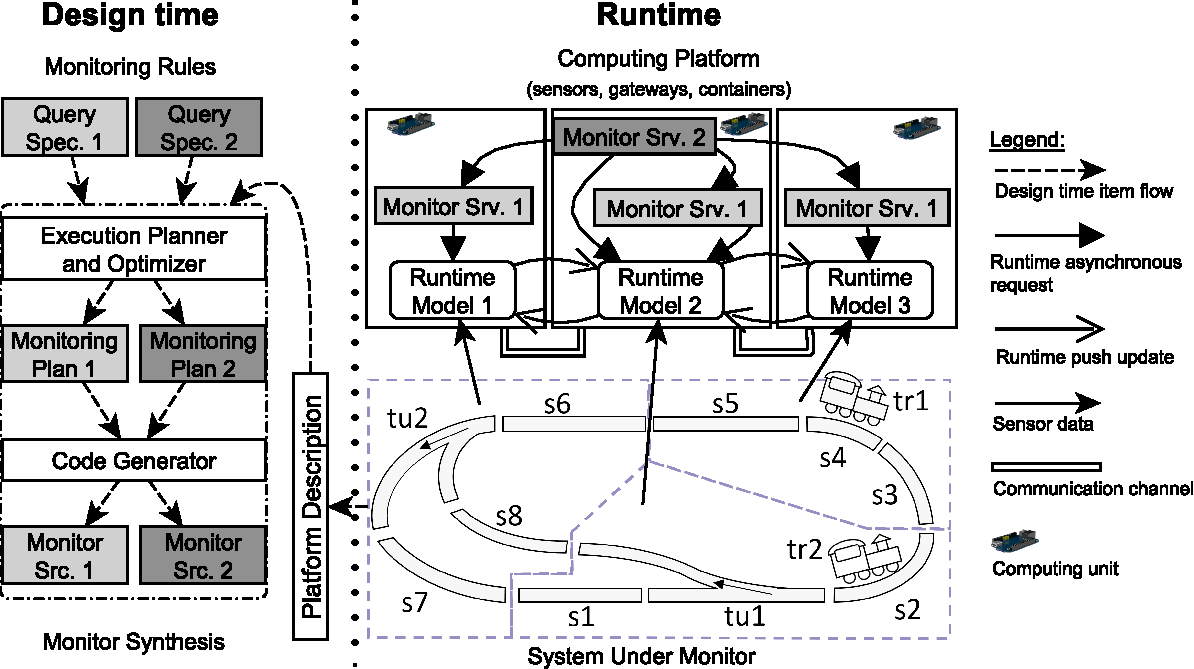
\includegraphics[width=\textwidth]{figures/fase-overview-crop.pdf}
		\caption{Approach for cyber-physical systems monitoring used by the presented framework }
		\label{fig:approach}
	\end{center}
\end{figure}

\subsection{Design time}

At first, the developer of the system must design the domain model of the CPS based on the structure of the target system.
From this domain model we generate the code that can be used to build up and maintain the live model of the system.

Then monitoring goals are defined as graph patterns. 
As patterns can refer to the meta model, it is a prerequisite for pattern definition. 
From these patterns we create monitoring plans. 
We use these plans to generate the source code of the monitoring components.

\subsection{Runtime}

At runtime, we rely on the generated monitor code and the generated model code. 
We create the nodes of the living model, create the references/edges between them and give the values of the attributes of the objects. 
With the physical world changing we update the objects to reflect the current state of the system. 
On this model, we run the monitoring code to find matches for the patterns in the model. 
If a pattern match occurs, we find the model elements that conform the pattern, thus we can locate the problems in the model, representing the cyber-physical system.


\section{Framework architecture}

Users of the framework can design the domain models of the system using EMF Ecore modeling.
Graph patterns can be defined using Viatra Query Language (VQL).
From this the framework creates the monitoring code, which is in \cpp{}.
Besides the generated code, the framework provides and additional library to  along with additional libraries, that are used by the generated code. 

\subsection{Code generation workflow}
EMF Ecore models and VQL files can be transformed into \cpp code by a set of Eclipse plugins.
These plugins are written in Xtend.
The workflow of code generation is depicted on \autoref{fig:workflow}

\begin{figure}[H]
	\begin{center}
		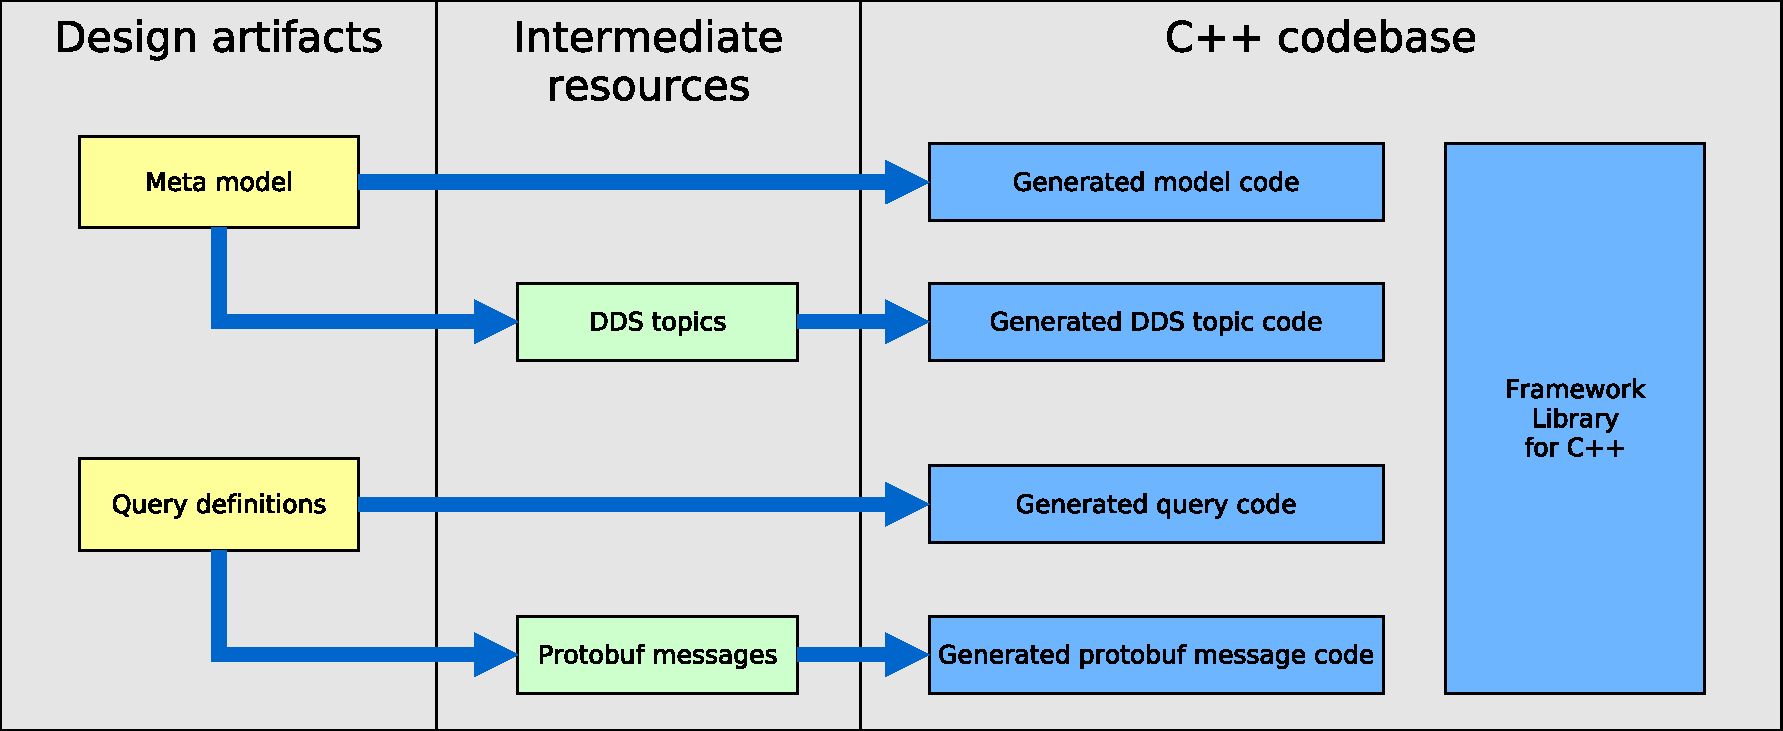
\includegraphics[width=\textwidth]{figures/workflow.pdf}
		\caption{ Model artifacts and their corresponding generated components }
		\label{fig:workflow}
	\end{center}
\end{figure}

From the EMF metamodel we generate model code, which can be used to build up and maintain the live model. 
We also generate the corresponding DDS topics, as DDS is used to notify computation units about object creation/deletion and reference creation/deletion.

From the VQL files we parse the graph patterns and generates the code able to execute them.
Query execution depends on serialization/deserialization service provided by protobuf, so we also create the corresponding protobuf messages and compiles them into \cpp{} code.

